\documentclass[12pt]{exam}
\usepackage{amsthm}
\usepackage{libertine}
\usepackage[utf8]{inputenc}
\usepackage[margin=1in]{geometry}
\usepackage{amsmath,amssymb}
\usepackage{multicol}
\usepackage[shortlabels]{enumitem}
\usepackage{siunitx}
\usepackage{cancel}
\usepackage{graphicx}
\usepackage{pgfplots}
\usepackage{listings}
\usepackage{tikz}
\usepackage{color, colortbl}
\usepackage{amsbsy}
\usepackage{pgfplots}

\pgfplotsset{compat=1.11}
\usetikzlibrary{calc}
\pgfplotsset{width=10cm,compat=1.9}
\usepgfplotslibrary{external}
\tikzexternalize
\graphicspath{ {./images/} }

\newcommand{\class}{High Performance Computing 1} % This is the name of the course 
\newcommand{\examnum}{Assignment 1: Write Up} % This is the name of the assignment
\newcommand{\examdate}{\today} % This is the due date
\newcommand{\timelimit}{}





\begin{document}
\pagestyle{plain}
\thispagestyle{empty}

\noindent
\begin{tabular*}{\textwidth}{l @{\extracolsep{\fill}} r @{\extracolsep{6pt}} l}
\textbf{\class} & \textbf{Name:} & \textit{Denzel Ayala}\\ %Your name here instead, obviously 
\textbf{\examnum} &&\\
\textbf{\examdate} &&\\
\end{tabular*}\\
\rule[2ex]{\textwidth}{2pt}
% ---


    \section*{\label{sec:prob1} Problem 1}

        For the fourth part of this problem I obtained all the residues from the provided output file. For the cumulative run time I used a for loop in \textbf{\textit{awk}} to add up all the provided times in the second to last column. In the case of count I gave two possible values. The first was the total number of rows extracted from the original file. The second count given was the addition of all the residues. Below is an image containing the commands I entered as well as the contents of the files requested. My code is slightly different from what is being displayed. For the screenshot I limited the residues gotten by grep using \textit{\ldots(002)}. In the submitted code every residue is printed to the file and the output count and runtime reflect that. 

        \begin{center}
            \includegraphics*[scale=0.4]{prob1.jpg}
        \end{center}

    \section*{\label{sec:prob2} Problem 2}

        \begin{enumerate} %You can make lists!

            \item \textbf{Specify Problem Requirements}

            The goal is to plot the Mandelbrot set by calculating series convergence (eq~\ref{eq:1}) at every point in a space. For this problem we will be working with complex numbers. They consist of a real and \textit{imaginary} component. These two components are orthogonal to each other. As a result the real and imaginary components can be treated as an $\hat{x}$ and $\hat{y}$ axis, respectively.
            \begin{center}
                \begin{gather}\label{eq:1}
                    z_{i} = z^{2}_{i-1} + c
                \end{gather}
            \end{center}

                 We are plotting within a range of $-2 \leq x \leq 2$ and $-1 \leq y \leq 1$. The plot range will be divided into individual points, that I will call \textbf{\textit{pixels}}, where convergence is tested. The ordered combination of the pixels form a mesh that determines the resolution power of the calculation. The plot on the left would be a representation of a low resolution mesh while on the left is a high resolution mesh. 

                 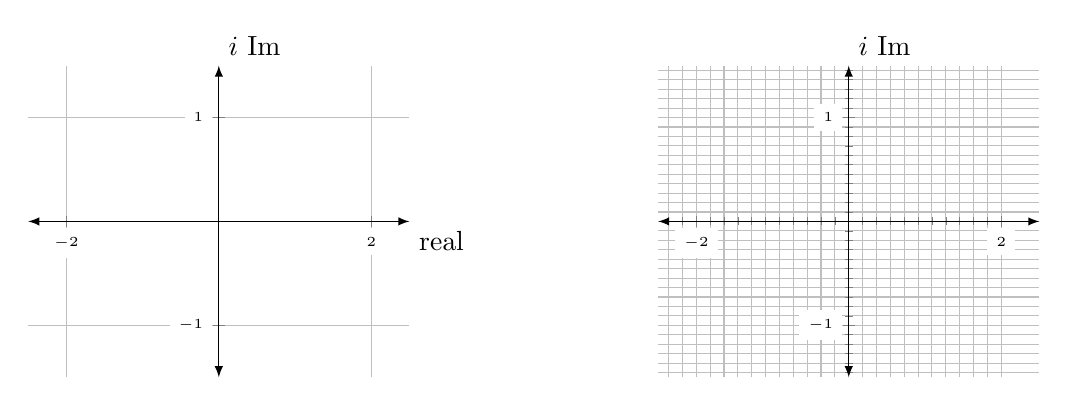
\begin{tikzpicture}
                    \begin{axis}[
                        xmin=-2,xmax=2,
                        ymin=-1,ymax=1,
                        grid=both,
                        axis lines=middle,
                        minor tick num=0,
                        enlargelimits={abs=0.5},
                        axis line style={latex-latex},
                        ticklabel style={font=\tiny,fill=white},
                        xlabel style={at={(ticklabel* cs:1)},anchor=north west},
                        ylabel style={at={(ticklabel* cs:1)},anchor=south west},
                        xlabel={real}, ylabel={$i$ Im},
                        width={0.55*\textwidth-7pt}
                    ]                   
                    \end{axis}
                
                    \begin{axis}[xshift=8cm,
                        xmin=-2,xmax=2,
                        ymin=-1,ymax=1,
                        grid=both,
                        axis lines=middle,
                        minor tick num=10,
                        enlargelimits={abs=0.5},
                        axis line style={latex-latex},
                        ticklabel style={font=\tiny,fill=white},
                        xlabel style={at={(ticklabel* cs:1)},anchor=north west},
                        ylabel style={at={(ticklabel* cs:1)},anchor=south west},
                        ylabel={$i$ Im},
                        width={0.55*\textwidth-7pt}
                    ]
                    \end{axis}
                \end{tikzpicture}
                    
                
                The convergence condition at a given pixel is $|z|\leq 2$. For understandability, an iteration will be a singular calculation of equation (\ref{eq:1}), where $z_i$ is the output of each iteration. A round will consist of iteration till divergence or assumed convergence after 1k-10k iterations. For the first iteration of each round $z_{i-1} = z_0 = 0$. Meanwhile, $c$ is given by the plot location of each pixel, or more tangibly each intersection (or square) in the plots above.

                The area is normally found by multiplying a length and a width. This would be difficult in the case of the Mandelbrot plot as its features are complex and very small. So a pixel count approach can be used to approximate the area of the curve.  


            \item \textbf{Analyze the Problem}
            
                The inputs to this system is the number of pixels in the real and imaginary directions. The output was initially a text file with a single binary (0 or 1) result for each pixel. In this initial output configuration a 0 indicated convergence while a 1 indicated the series diverted at that point c. This was modified later to be an unsigned integer where the value of the integer indicates how many iterations it took to break the boundary condition. This modification was made to include color into the plots produced

                The area input is the vector that holds all the pixel values. The output is a count of 0's in the vector divided by the total number of pixels.



            \item \textbf{Design the Algorithm}
            
                Below is the general architecture of the program:

                Main()$\lbrace$ \\
                    call mesh-generator(x-res, y-res, vector) \\
                    call area-finder(vector) \\
                $\rbrace$
                
                mesh-generator()$\lbrace$ \\
                    for y in range -2,2 $\lbrace$

                    for x in range -1,1 $\lbrace$
                        calc-series-convergence(c)

                $\rbrace \rbrace \rbrace$

                area-finder()$\lbrace$
                for integer in each vector cell$\lbrace$
                    if integer == 0 count+=1 $\rbrace$ 

                count/vector-size
                $\rbrace$


            \item \textbf{Implement the Algorithm / Test and Verify the Completed Program}
            
                The algorithm compiled and ran. The output text files were put into python and turned into matrices that were plotted using matplotlib in python. 

                \begin{center}
                \begin{tikzpicture}
                    \begin{axis}[
                        xmode=log,
                        log ticks with fixed point,
                        xlabel={Resolution (pixels)},
                        ylabel={Area}
                    ]
                    \addplot table {
                    10 2.880
                    100 1.910
                    1000 1.859
                    };
                    \end{axis}
                    \end{tikzpicture}
                \end{center}
            

        \end{enumerate}



                HIGH SPIN AND LOW SPIN STATES INORGANIC CHEMISTRY USE GROUP THEORY AND CRYSTAL FIELD THEORY TO DESCRIBE THIS. HUNDS RULE VS PAULI EXCLUSION TUNABILITY USING \ldots

            
            \begin{gather*}
                n \: \text{bits} = \left(x \: \text{bytes}\right) \left(y \: \frac{\text{bits}}{\text{byte}}\right) \\
                \text{MAX\_RANGE} = 2^{n}
            \end{gather*}

            

        
    \section*{\label{sec:prob3} Problem 3}

    \section*{\label{sec:prob4} Problem 4}


\end{document}